\subsection{轨迹停留点检测}
现实生活中用户的日常轨迹通常是有一系列包含了地理坐标和时间戳的GPS位置点构成,每个坐标点包含了详细的经纬度、时间戳信息、海拔高度、移动速度等信息。如图\ref{fig:2_1}所示。我们可以通过一些算法检测出用户在一段轨迹运动中停留过的地方称之为停留点\upcite{zheng2011computing},本文的停留点并不是指运动速度静止的点,而是由一系列GPS点构成的。如图\ref{fig:2_1}中$p_{4} \sim p_{8}$构成了一个停留点stay point在图中由红色点表示。这个点表示用户在该区域内的停留时间超过了一个设定的时间阈值$\Delta T$,相比于用户的其他轨迹位置点,这些计算得出的停留点蕴含了更重要的信息,通过语义标签甚至可以得出用户去过某家餐馆和电影院等。基于以上理论,用户的GPS位置轨迹可以转换为一组由停留点所组成的序列,如$sp_{1}\overset{\Delta_{t1}}{\rightarrow} sp_{2}\overset{\Delta_{t2}}{\rightarrow}\cdots \overset{\Delta_{tn-1}}{\rightarrow}sp_{n}$,这样由停留点所表示的序列不仅对原有数据维度进行了压缩,同时也保存了用户的重要信息。
\begin{figure}[H]
\centering
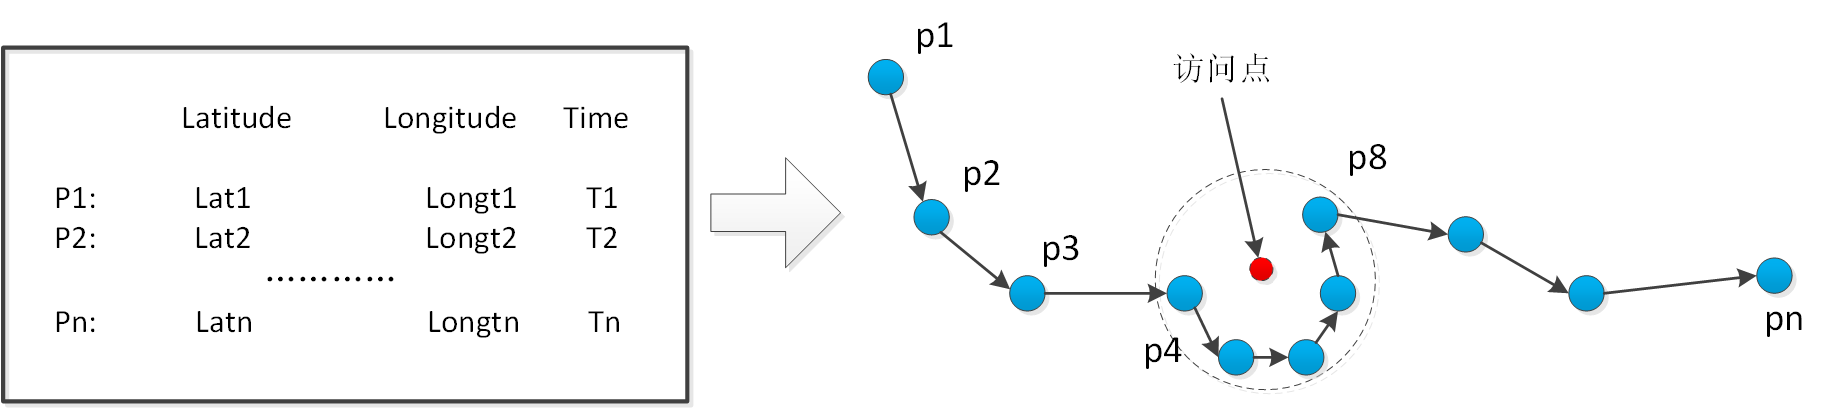
\includegraphics[width=0.8\textwidth]{figure2_1_gps}
\caption{用户GPS轨迹示例图}
\label{fig:2_1}
\end{figure}
\par 停留点的计算过程如算法\ref{alg2_1staypoint}所示。
\begin{algorithm}[htb]
\caption{停留点检测算法}
\label{alg2_1staypoint}
\begin{algorithmic}[1] %每行显示行号
				\REQUIRE 用户GPS轨迹 $Tra$,$\Delta T$,$\Delta_{distance}$
				\ENSURE 用户停留点序列$SP$
				%\Function {SPDec}{$Tra, \tau_{time},\tau_{distance}$}
				\STATE $i = 0$ , $PointNum= \left| \ Tra \right|$,$SP = Null$
				\WHILE {$i<PointNum$}
				\STATE $j = i+1$
				\WHILE {$j < PointNum$}
				\STATE $distance=Dis(Tra_{i},Tra_{j})$
				\IF {$distance > \Delta_{distance}$}
				\STATE $\Delta_{t}=Tra_{j}.T-Tra_{i}.T$
				\IF {$\Delta_{t} > \tau_{time}  $ }
				\STATE $p.Lat = avg(Tra_{k}.Lat)  $
				\STATE $p.Lng = avg(Tra_{k}.Lng)$
				\STATE $p.T = Tra_{i}.T(arv|lev)$%p.levT = Tra_{j}.T $
				\STATE $SP .add(p) ;j++; $
				\ENDIF				
				\ENDIF				
				\ENDWHILE
				\STATE $i=j ; break$
				\ENDWHILE
				\STATE \RETURN {$SP$}
				%\EndFunction				
\end{algorithmic}
\end{algorithm}

--------------------------------------------------------------------------------
\chapter{RSMHD用户关系强度计算框架模型}
\label{chap:chapter07}
上一章详细介绍了和本研究数据源相关的处理技术与方法,接下来这一章将主要介绍RSMHD的多维据源多维度的关系度量模型的整体框架结构。
\section{RSMHD模型框架描述}
\label{sec:section7-1}
本研究的主要内容是通过采集到的用户感知数据(GPS轨迹信息 、WiFi数据、蓝牙数据)来开展用户之间的关系强度度量工作。因此本文希望能够提供一种基于此类非社交的感知数据建立的通用的用户关系强度计算框架。非社交数据主要是指不是来自于用户直接社交活动中所收集到的数据,在本研究中主要包含了用户轨迹数据、用户WiFi感知数据和用户蓝牙感知数据。因此本课题基于以上三种不同的感知数据源提出了能够统一处理多种数据源的计算框架,其整体概要结构图如图\ref{fig:7_1}所示,图中描述整体架构由以下几部分组成:上下文感知收集模块、基于用户日常轨迹的关系强度计算模块、基于用户WiFi感知数据的关系强度计算模块和基于用户蓝牙的关系强度计算模块。用户的日常语义轨迹是有连续的GPS位置点所组成的轨迹的集合,在用户的轨迹信息的采集过程中,因受到地形、气候、GPS 传感器的干扰误差的影响,会出现GPS漂移现象,GPS的位置漂移使得用户的轨迹数据中存在大量的噪音数据,影响后续对数据的处理和分析。因此对采集到的用户轨迹数据采取滤波处理,消除轨迹中所蕴含的噪音数据。GPS 位置的采集还受到地形环境的影响,在室内无法获取GPS 位置信息的时候会导致用户轨迹的缺失,造成计算结果产生巨大偏差。第四章部分将重点针对上述问题展开GPS轨迹的处理研究工作,以获得好的信息效果。对于剩余的WiFi和蓝牙感知数据来讲,主要的工作是针对二者数据源的特点以及后续的算法输入对原始数据进行提取和结构化建模表示存储。第四章的其余部分将会针对WiFi和蓝牙感知数据的预处理和结构化表示进行详细的描述。
\begin{figure}[htp]
\centering
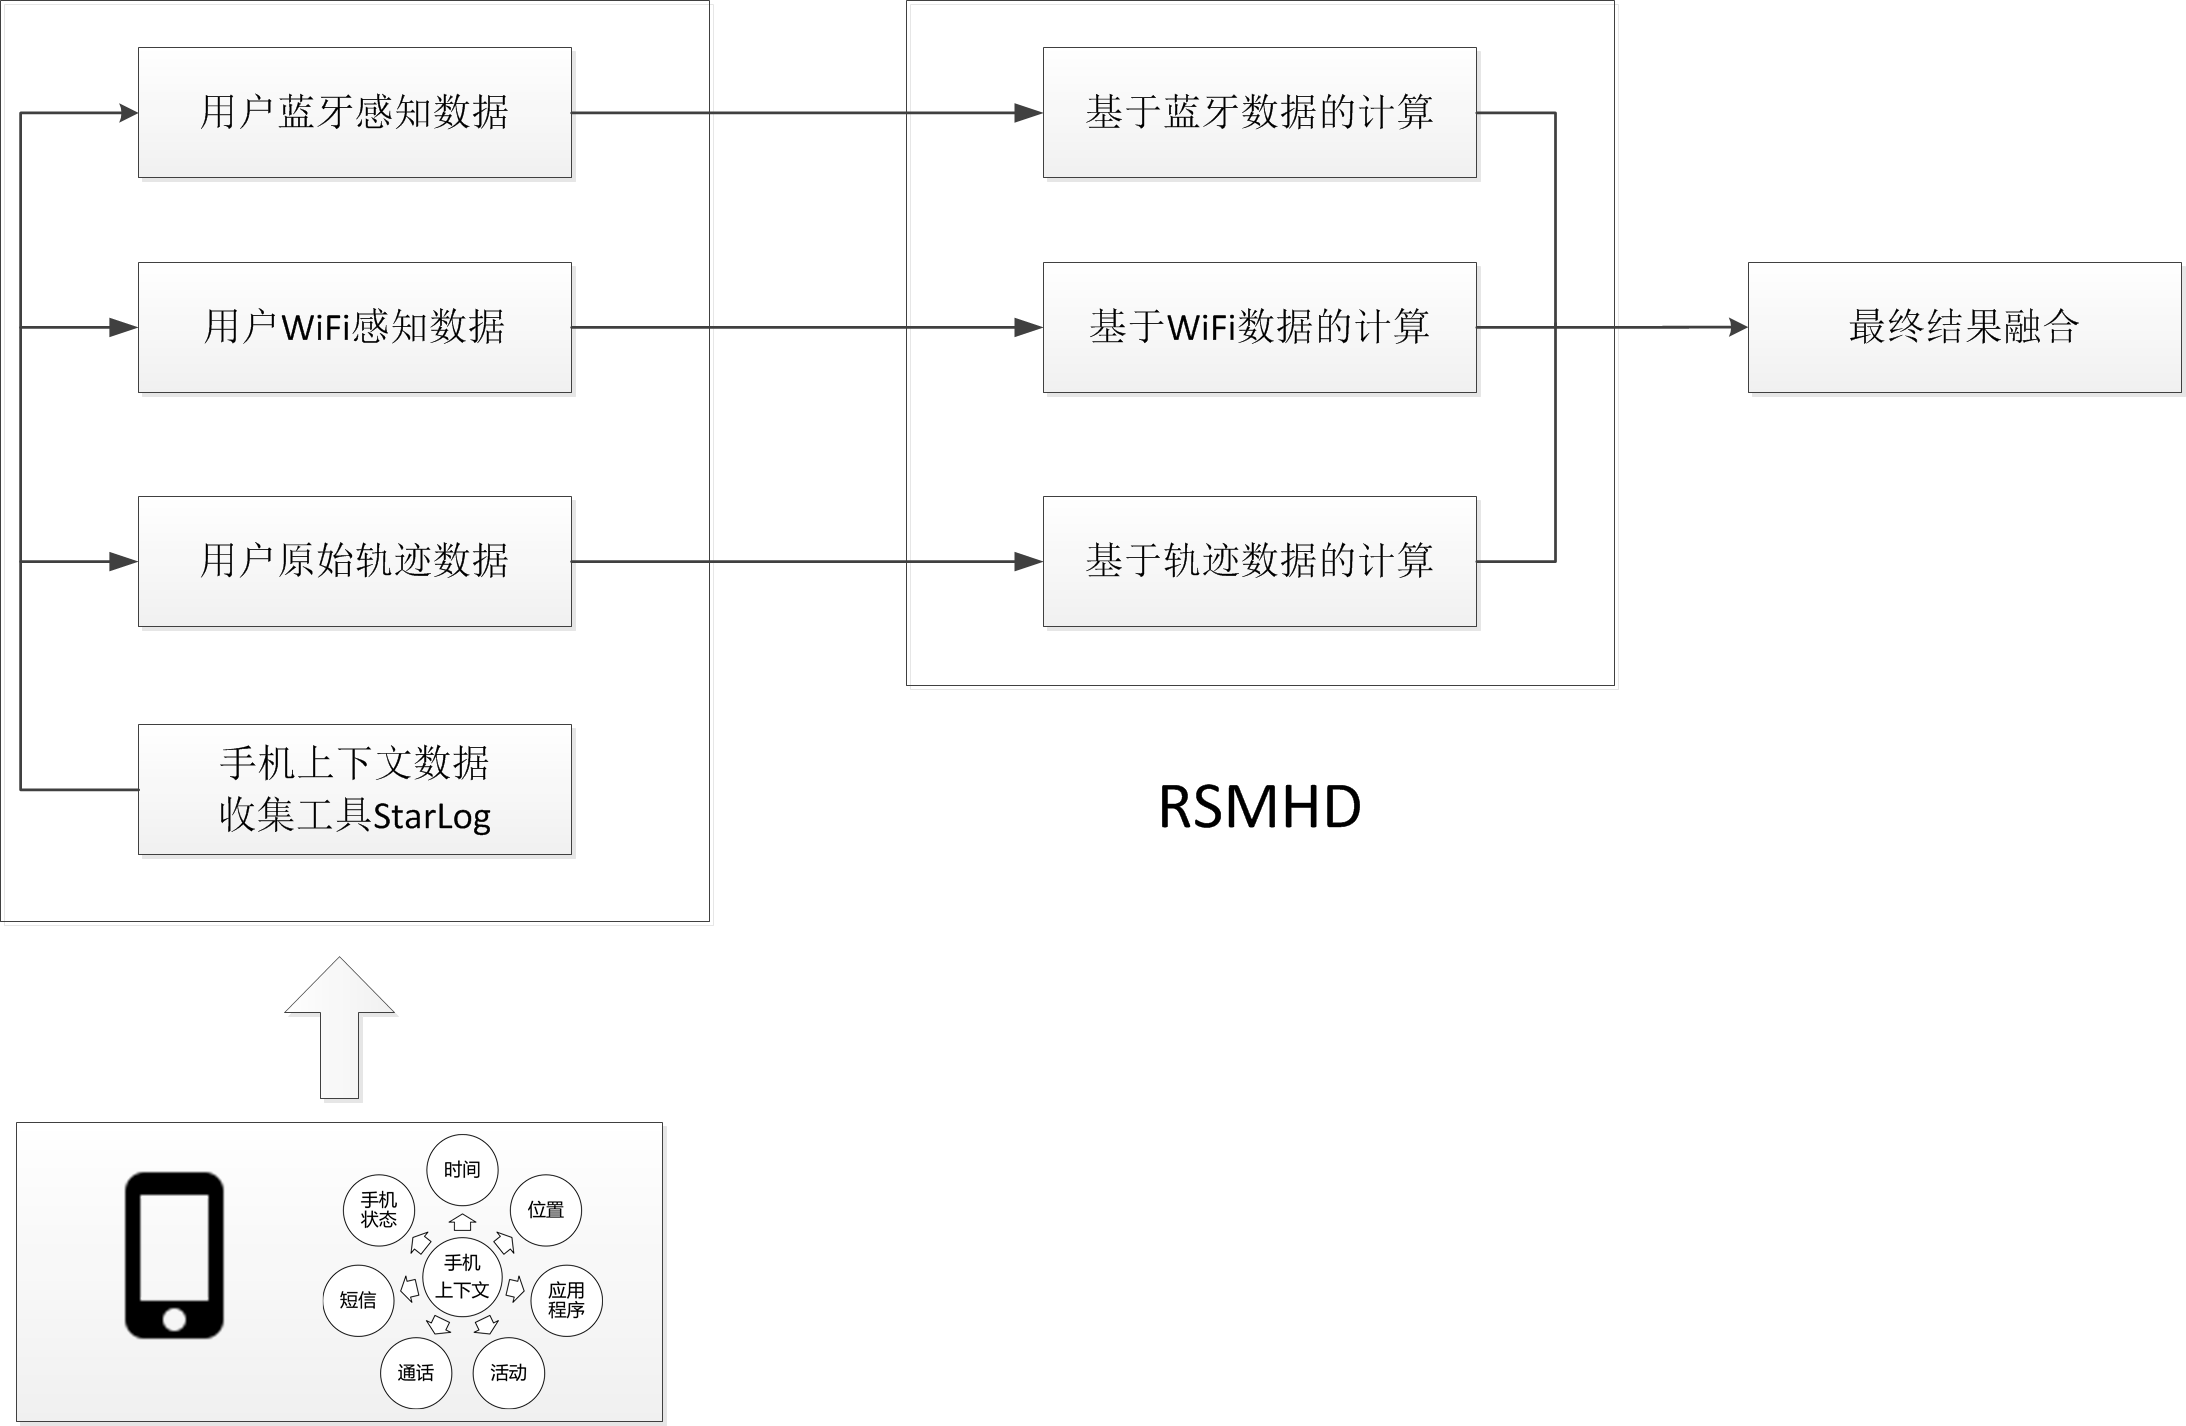
\includegraphics[width=0.8\textwidth]{figure7_1_RSMHD}
\caption{RSMHD用户关系强度计算模型框架图}
\label{fig:7_1}
\end{figure}
\subsection{基于轨迹数据的关系强度计算模块概述}
在本研究中所提出的RSMHD计算框架模型中,第二层需要基于用户的日常语义轨迹分别通过计算地理轨迹相似性、用户的语义轨迹相似性以及日常轨迹运动模式三个层次关系强度融合为轨迹强度结算结果,其详细框架图如图\ref{fig:7_1_tra}所示。在这个模块中,通过计算用户日常地理轨迹的相似性推测出用户之间的关系强度;针对用户活动产生的日常语义轨迹,RSMHD 模型采利用自然语言处理的思想,通过快速编码变换计算出用户基于语义轨迹的关系强度;第三层中,RSMHD 进一步挖掘出用户轨迹中更高一层的上下文信息(High Context)得出用户日常轨迹模式如:用户A 经常喜欢到校外某地用餐、用户B 经常下午在操场跑步等这些代表用户日常轨迹活动模式的信息,计算用户之间基于运动模式的关系强度。
\begin{figure}[htp]
\centering
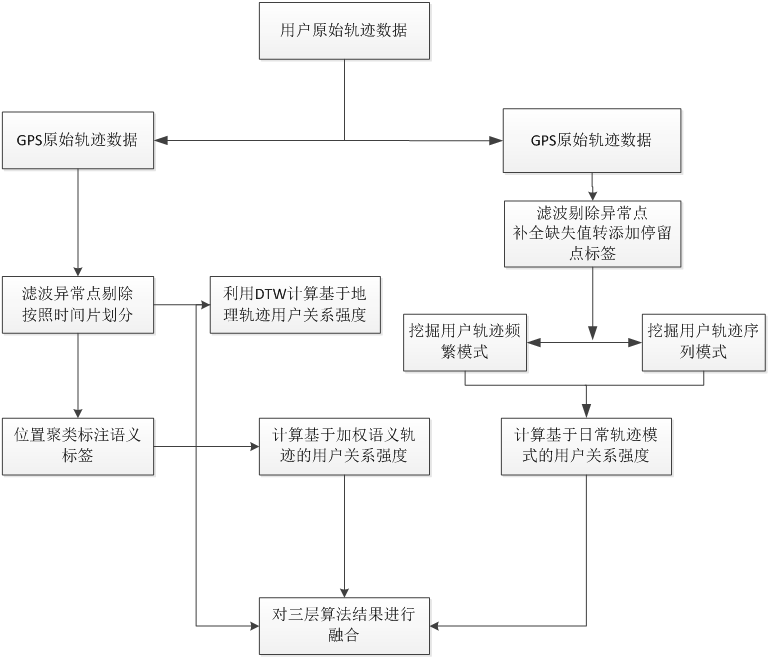
\includegraphics[width=0.8\textwidth]{figure7_1_tra}
\caption{RSMHD中基于用户轨迹计算模块详细框架图}
\label{fig:7_1_tra}
\end{figure}
\subsection{基于WiFi和蓝牙数据的关系强度计算模块概述}
在RSMHD计算框架模型中我们针对WiFi和蓝牙原始数据的特点以及现实生活中WiFi和蓝牙上下文环境的特征,采用了区别于原有基于WiFi和蓝牙计算社交关系的方法,整体的详细计算框架如图\ref{fig:7_1_wifi}所示。在WiFi和蓝牙数据处理计算框架中,分别针对底层手机的上下文感知信息进行数据信息的提取的规整,从复杂冗余的信息中萃取出关键的富有价值的信息;然后结合WiFi和蓝牙各自的上下文环境特征信息,将整理后的数据用图的数据结构进行结构化表示,使得抽象表示后的数据结构更加符合现实中的含义;最后基于结构化后的感知数据进行关系强度计算,将结果输出到下一层。
\begin{figure}[htp]
\centering
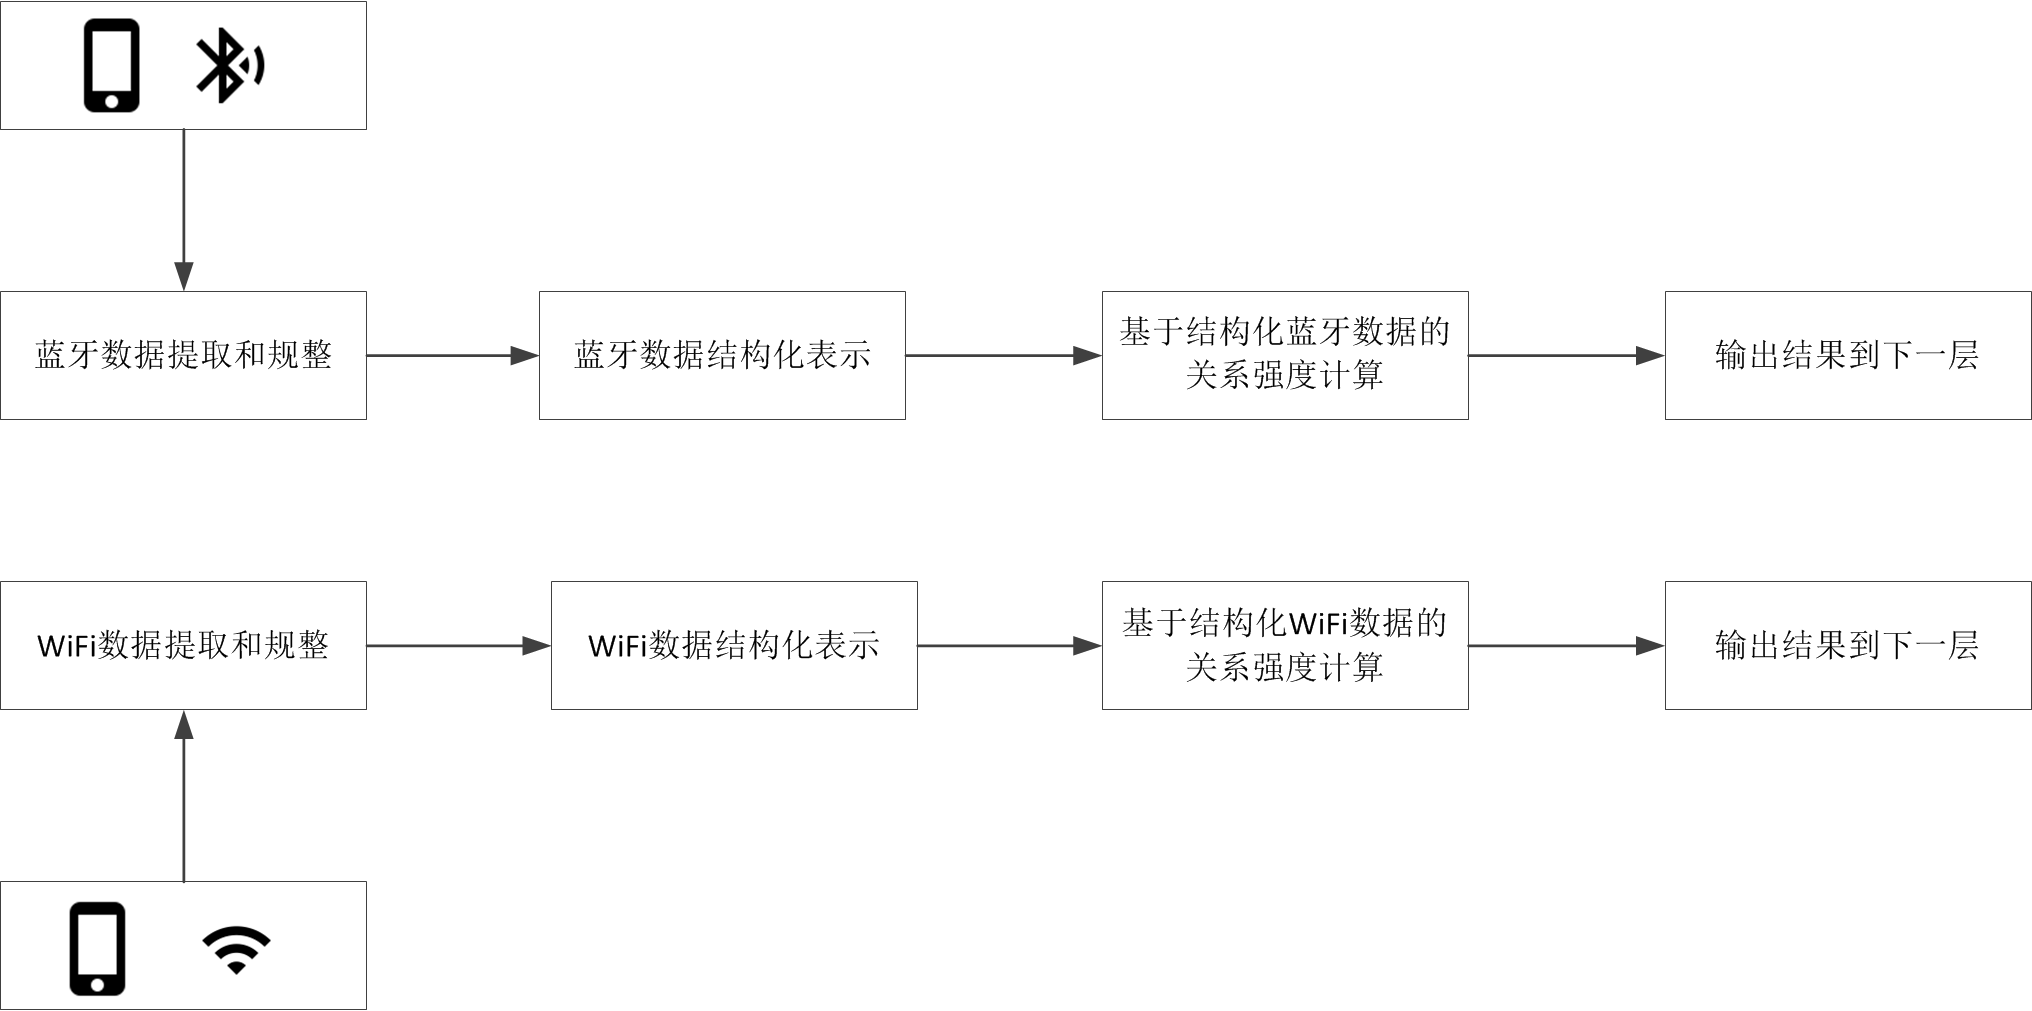
\includegraphics[width=0.8\textwidth]{figure_3_RSMHDwifibluee}
\caption{RSMHD中基于WiFi和蓝牙计算模块详细框架图}
\label{fig:7_1_wifi}
\end{figure}
\section{RSMHD模型计算流程概述}
\label{sec:section7-2}
整个信息采集是采用我们自己编写的用户手机上下文信息收集工具StarLog来记录保存用户手机的上下文感知数据如:GPS位置信息、WiFi感知信息、蓝牙感知信息、脱敏的通话记录、短信记录、APP使用记录等。
\par 针对用户的GPS位置数据我们首先对轨迹数据进行预处理,即采用滤波算法检测出用户日常轨迹中的漂移点减少轨迹中的噪音;然后根据停留点检测算法识别出用户轨迹中的停留点,针对缺失的轨迹点进行预测补全;第一层次中针对用户日常空间轨迹相似性计算时,可用将每天的轨迹数据划分为若干时间片的数据,然后采用DTW加权算法对时间片内的空间轨迹相似度进行计算并按照一天的轨迹进行处理。对于基于用户语义轨迹推倒关系强度这层我们首先将得到的停留点进行聚类分析,得到聚类后的停留点集合因此对于每一个簇都是同一个语义位置,然后将聚类GPS转换为现实社会中的语义标签,在计算用户语义轨迹的相似性时,采用快速hash算法将用户分片后的语义轨迹序列作为输入,得到用户之间每天的语义轨迹相似度,以及最终的语义轨迹相似度并将结果作为用户自己的关系强度。在上一层的基础上,我们针对得到的用户语义估计进行挖掘,寻找出用户的日常运动模式,然后计算用户运动模式之间的相似度并作为关系强度之一进行输出,综合三层的计算结果得到用户基于轨迹数据计算得到的关系强度。
\par 其次针对用户的WiFi和蓝牙数据,首先从原始数据中提取出重要的信息,并将WiFi和蓝牙数据进行结构化存储处理,采用图的存储结构,将WiFi和蓝牙数据还原为现实生活中的存在环境,然后针对用户切片时间内每刻的感知环境进行相似度计算,并将一天中的计算结果进行汇总进一步得到所有时间段内的用户相似度,最后将结果作为基于两种数据源推测出的用户关系强度。
\par 最后,在基于前面三种数据源的用户关系强度计算结果的基础上,采用集成学习的思想对计算结果进行融合处理,得到最终的用户关系强度计算结果。

-------------------------------------------------------------------------------------------------------------------------------------
\subsection{剔除轨迹中的异常点}
前文已经提到,由于在获取GPS位置信息的时候会受到位置漂移的影响,导致在获取用户实际位置的时候可能产生采样的误差甚至跳跃,为了使得最终计算得到的关系强度结果更为准确我们需要对GPS轨迹数据进行滤波分析。在第二章中描述了常用的三种滤波方法,在本章中将会针对三种滤波算法进行最后结果展示并根据结果分析最终采用此滤波算法的原因。
\par 首先接下来使用我们自己开发的用户感知数据收集软件StarLog,来分析观察各种滤波算法对用户轨迹中异常点检测剔除的效果,如图如图\ref{fig:3_2_1}、\ref{fig:3_2_2}所示。
\begin{figure}[htb]
  \centering%
  \subfloat[原始轨迹数据]{%
    \label{fig:3_2_1_1}
    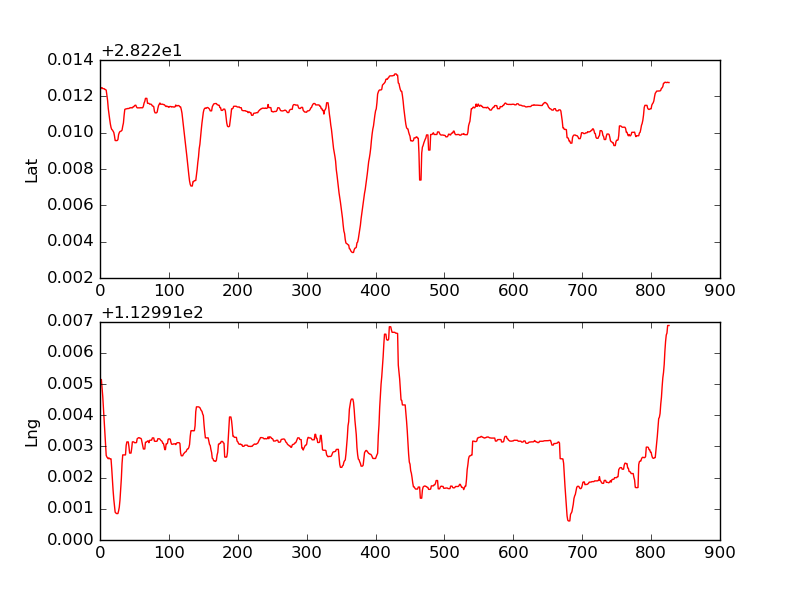
\includegraphics[height=4cm]{figure_4_mid_location1}}\hspace{4em}%
  \subfloat[中值滤波后的轨迹数据]{%
    \label{fig:3_2_2_1}
    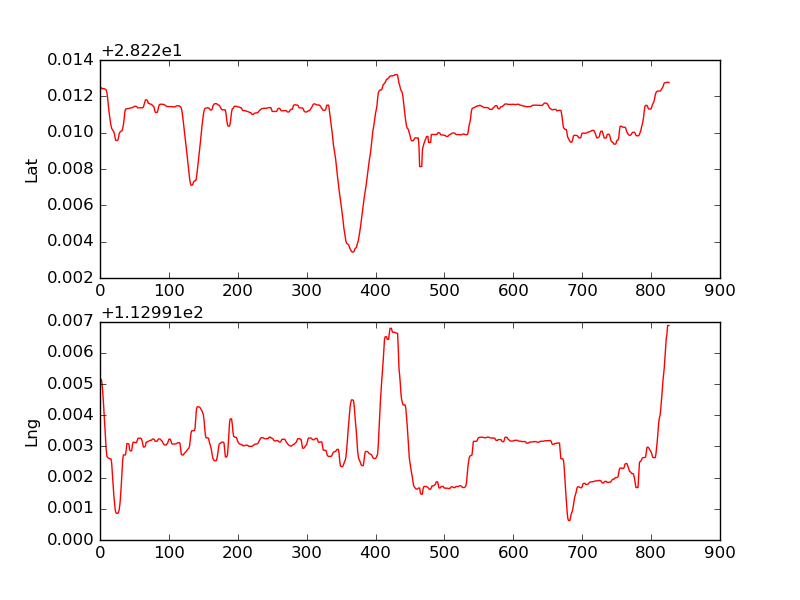
\includegraphics[height=4cm]{figure_4_mid_location1_ed}}
  \caption{轨迹中值滤波实验结果1}
  \label{fig:3_2_1}
\end{figure}
\begin{figure}[htb]
  \centering%
  \subfloat[原始轨迹数据]{%
    \label{fig:3_2_2_1}
    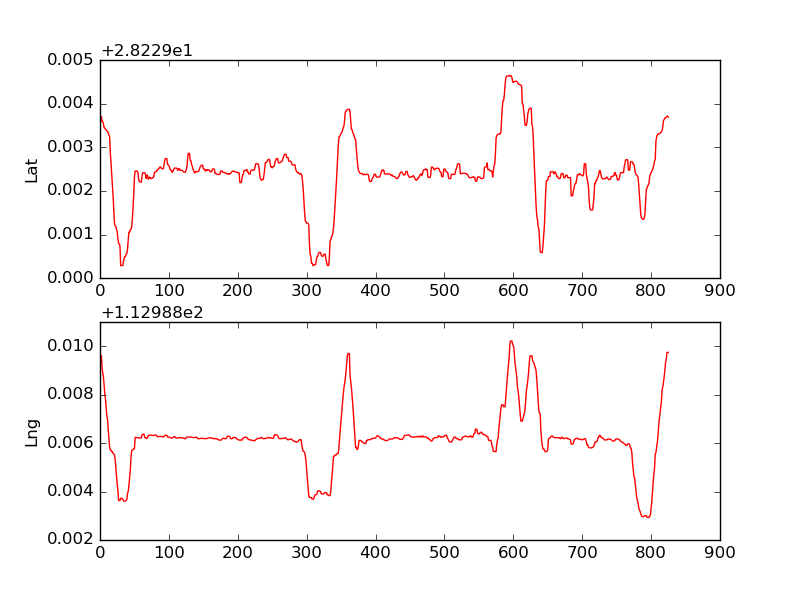
\includegraphics[height=4cm]{figure_4_mid_location2}}\hspace{4em}%
  \subfloat[中值滤波后的轨迹数据]{%
    \label{fig:3_2_2_2}
    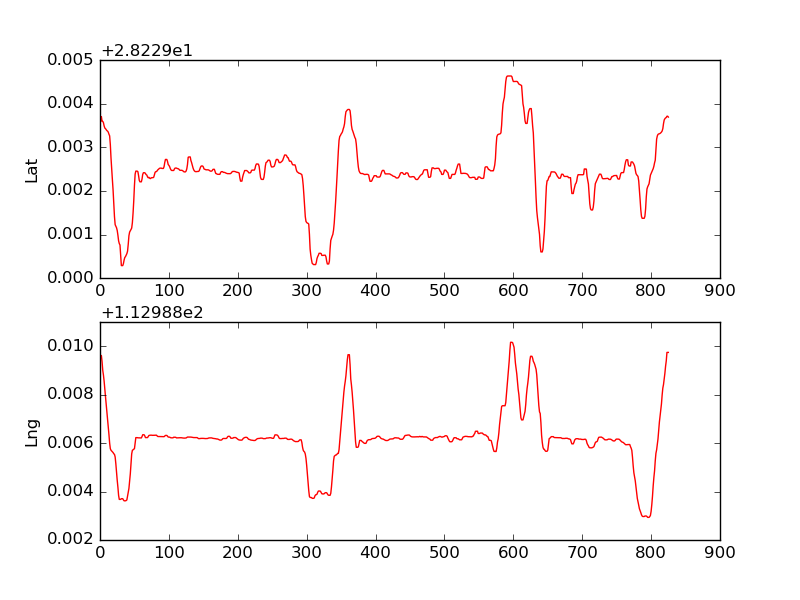
\includegraphics[height=4cm]{figure_4_mid_location2_ed}}
  \caption{轨迹中值滤波实验结果2}
  \label{fig:3_2_2}
\end{figure}
\par 从实验结果中我们可以观察到虽然中值滤波能够过滤掉其中少部分的位置漂移点,但是针对于一些明显的轨漂移点却没有能够很有效的识别过滤。
\par 接下来我们再使用均值滤波算法对用户轨迹进行分析,观察均值滤波算法对用户轨迹中异常点的检测情况,部分实验结果见图图\ref{fig:3_3_1}、\ref{fig:3_3_2}。
\begin{figure}[htb]
  \centering%
  \subfloat[原始轨迹数据]{%
    \label{fig:3_2_1_1}
    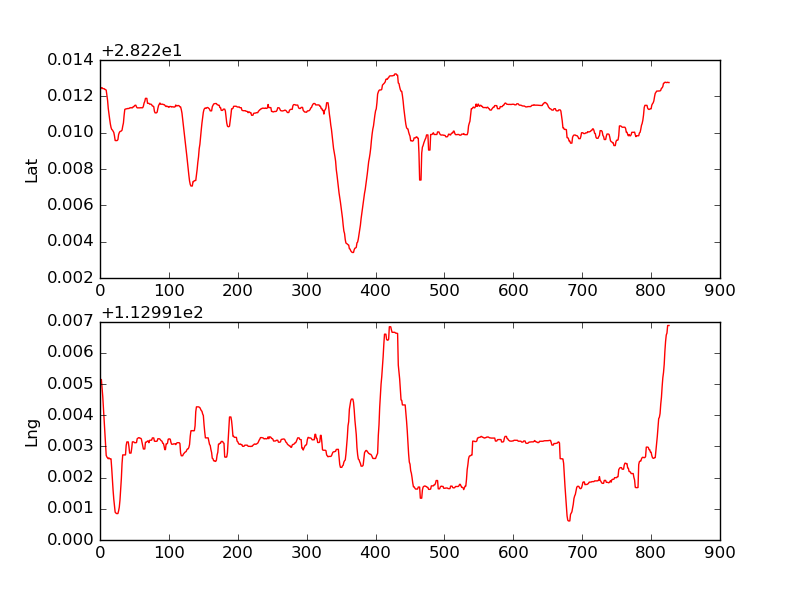
\includegraphics[height=4cm]{figure_4_mid_location1}}\hspace{4em}%
  \subfloat[均值滤波后的轨迹数据]{%
    \label{fig:3_2_2_1}
    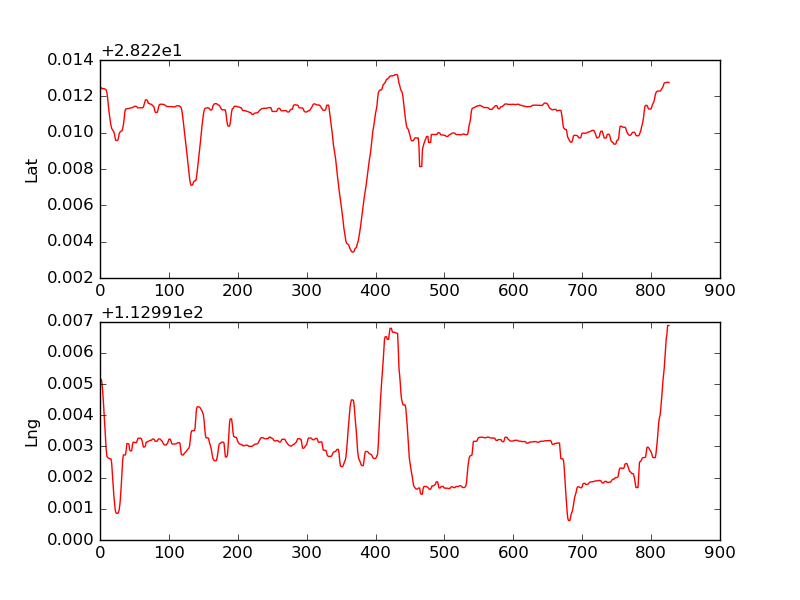
\includegraphics[height=4cm]{figure_4_mid_location1_avg}}
  \caption{轨迹均值滤波实验结果1}
  \label{fig:3_3_1}
\end{figure}
\begin{figure}[htb]
  \centering%
  \subfloat[原始轨迹数据]{%
    \label{fig:3_2_2_1}
    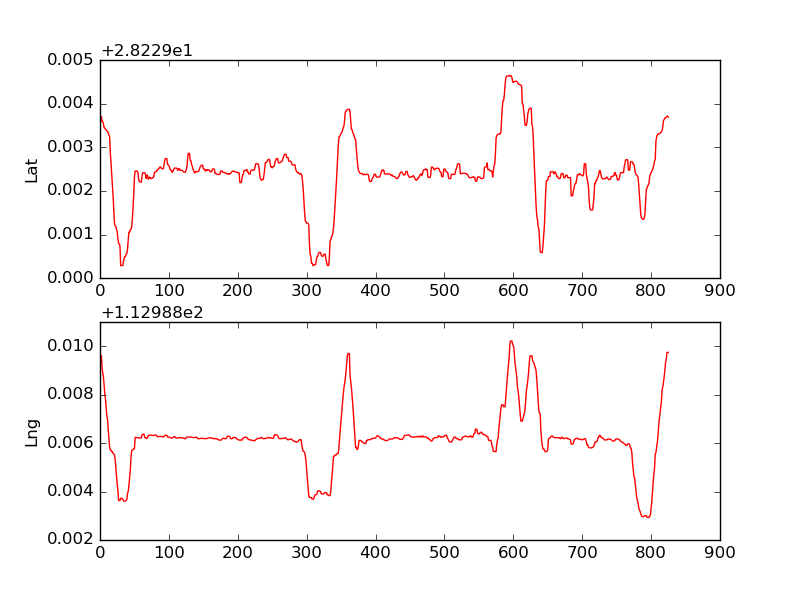
\includegraphics[height=4cm]{figure_4_mid_location2}}\hspace{4em}%
  \subfloat[均值滤波后的轨迹数据]{%
    \label{fig:3_2_2_2}
    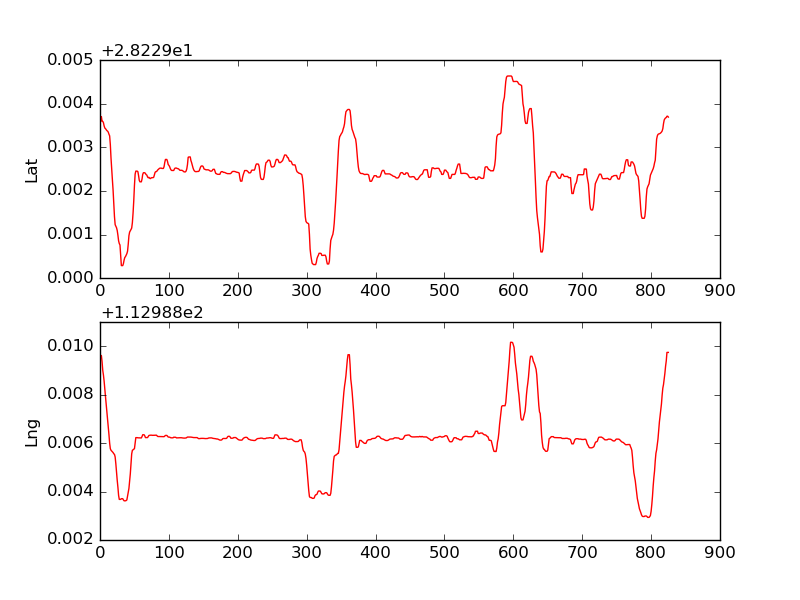
\includegraphics[height=4cm]{figure_4_mid_location2_avg}}
  \caption{轨迹均值滤波实验结果2}
  \label{fig:3_3_2}
\end{figure}
\par 通过对比观察滤波结果图可以发现,相对于中值滤波,均值滤波能够较好的平滑用户的轨迹变化曲线,剔除GPS漂移点。但是,同样无法很有效的处理漂移偏差大的位置点。
\par 通过采取卡尔曼滤波算法得到的用户轨迹如图\ref{fig:3_4_1}、\ref{fig:3_4_2},根据观察图中滤波后的用户轨迹数据,我们可以发现虽然图形变得平滑了许多,但是却使得原有的轨迹信息收到了模糊,难以有效的将两个用户轨迹进行相似度计算。
\begin{figure}[htb]
  \centering%
  \subfloat[原始轨迹数据]{%
    \label{fig:3_2_1_1}
    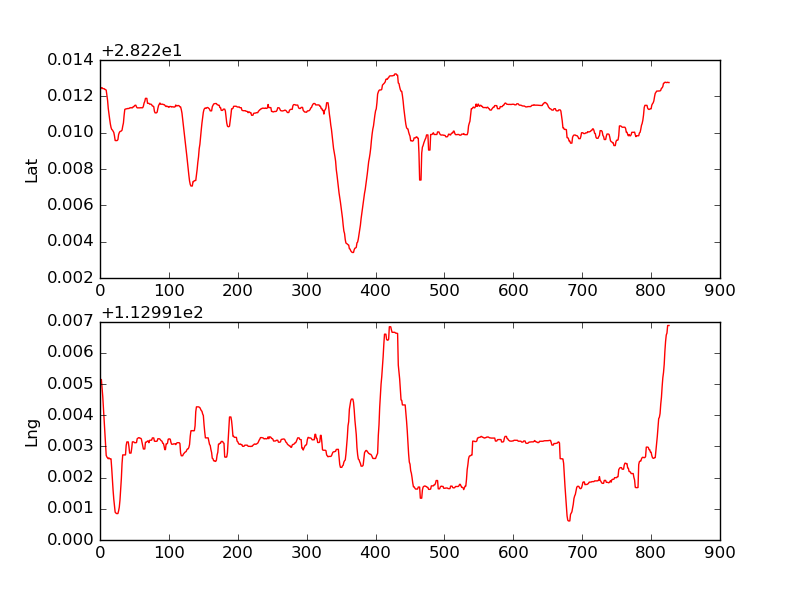
\includegraphics[height=4cm]{figure_4_mid_location1}}\hspace{4em}%
  \subfloat[卡尔曼滤波后的轨迹数据]{%
    \label{fig:3_2_2_1}
    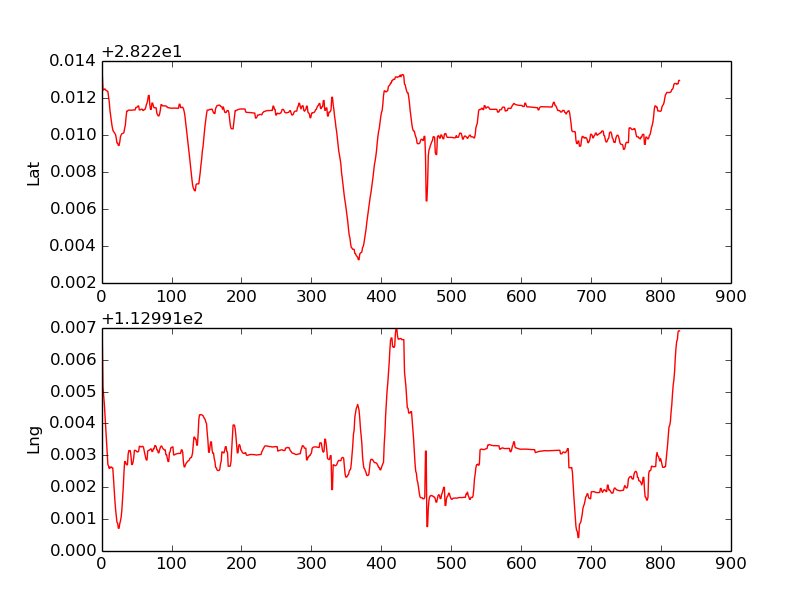
\includegraphics[height=4cm]{figure_4_mid_location1_kalman_ed}}
  \caption{卡尔曼滤波实验结果1}
  \label{fig:3_4_1}
\end{figure}
\begin{figure}[htb]
  \centering%
  \subfloat[原始轨迹数据]{%
    \label{fig:3_2_2_1}
    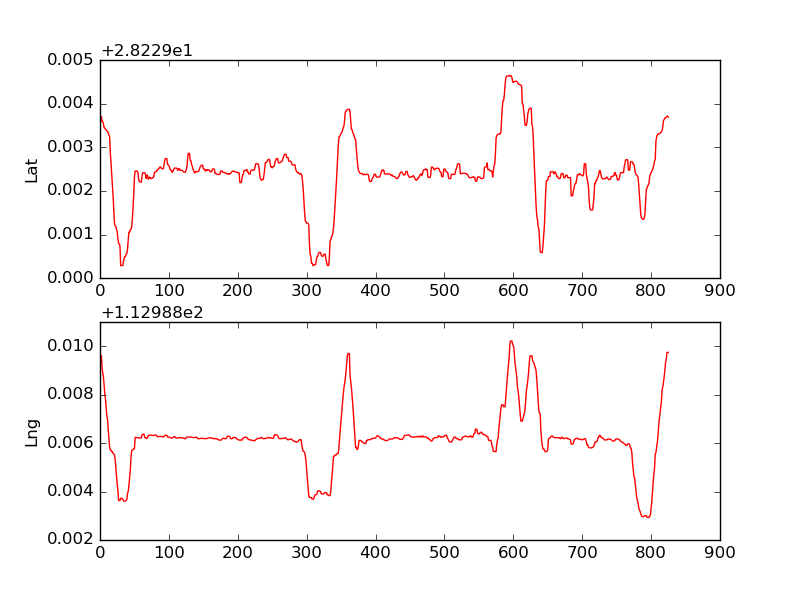
\includegraphics[height=4cm]{figure_4_mid_location2}}\hspace{4em}%
  \subfloat[卡尔曼滤波后的轨迹数据]{%
    \label{fig:3_2_2_2}
    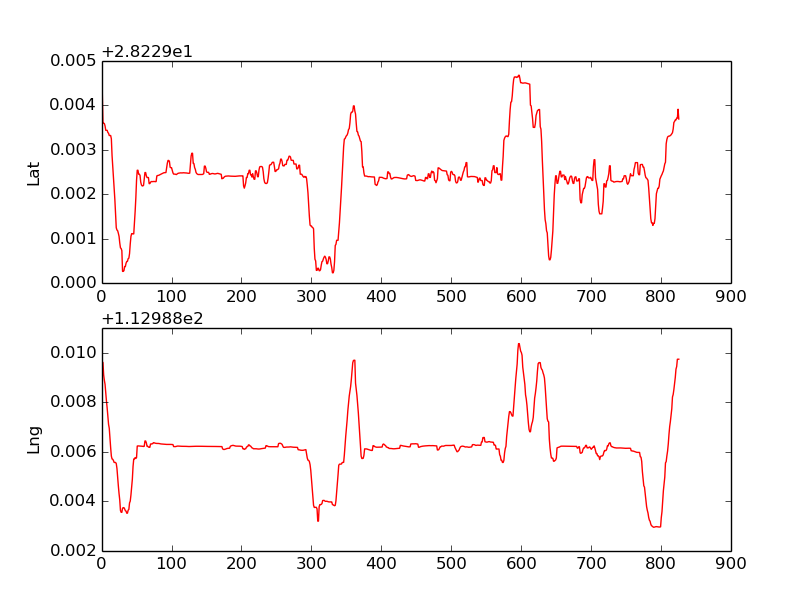
\includegraphics[height=4cm]{figure_4_mid_location2_kalman_ed}}
  \caption{卡尔曼滤波实验结果2}
  \label{fig:3_4_2}
\end{figure}
\par 在本研究中,我们采用了一种基于速度的分段卡尔曼滤波方法。考虑到在一个时间片内,如果当前位置点的速度和它之前的位置点的速度绝对差大于$\Delta v$ 时($\Delta v$作为一个未知的参数,需要我们在实际使用中给出)采用这样的方法将原有用户轨迹切分为$n$段然后针对每一段轨迹采用卡尔曼滤波算法,最终的部分轨迹滤波结果见图\ref{fig:3_5_1}、\ref{fig:3_5_2},可见经过按照速度分段后使用卡尔曼滤波能够比较好的过滤掉漂移点。
\begin{figure}[htb]
  \centering%
  \subfloat[原始轨迹数据]{%
    \label{fig:3_2_1_1}
    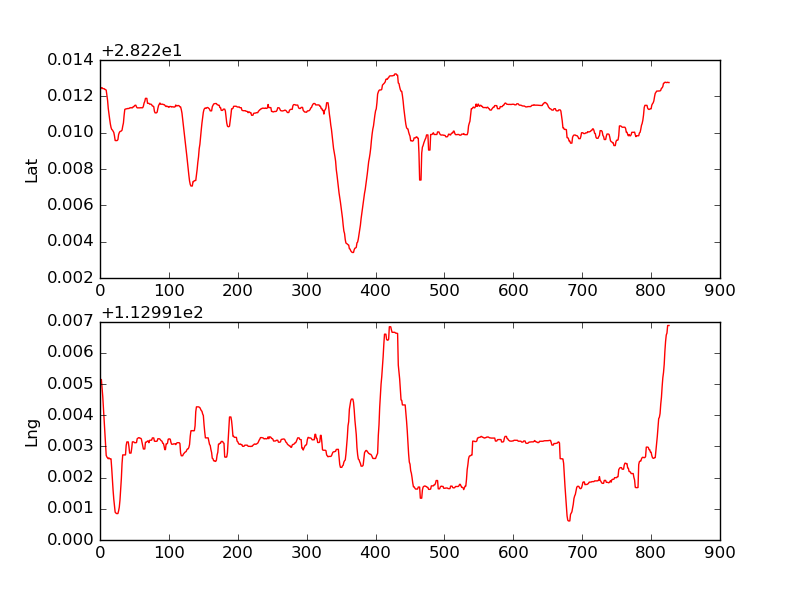
\includegraphics[height=4cm]{figure_4_mid_location1}}\hspace{4em}%
  \subfloat[分段卡尔曼滤波数据]{%
    \label{fig:3_2_2_1}
    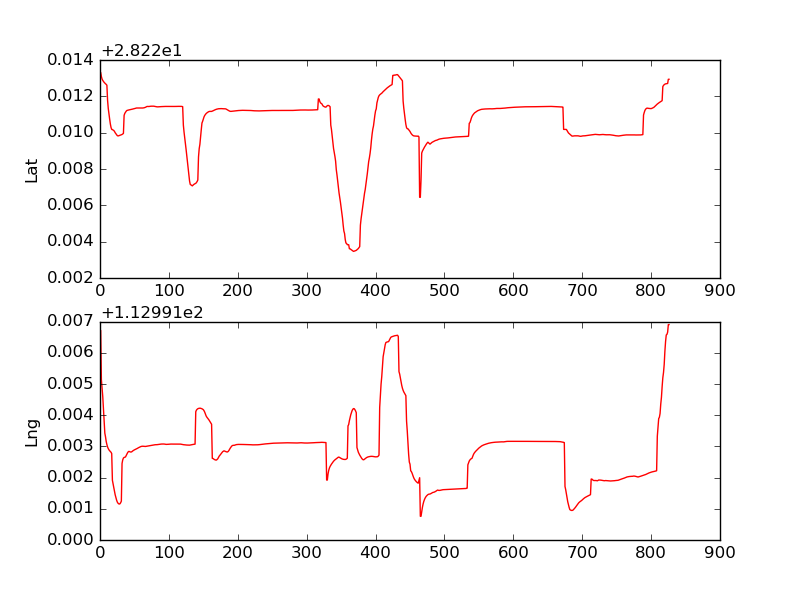
\includegraphics[height=4cm]{figure_4_mid_location1_kalman}}
  \caption{分段卡尔曼滤波轨迹结果1}
  \label{fig:3_5_1}
\end{figure}
\begin{figure}[htb]
  \centering%
  \subfloat[原始轨迹数据]{%
    \label{fig:3_2_2_1}
    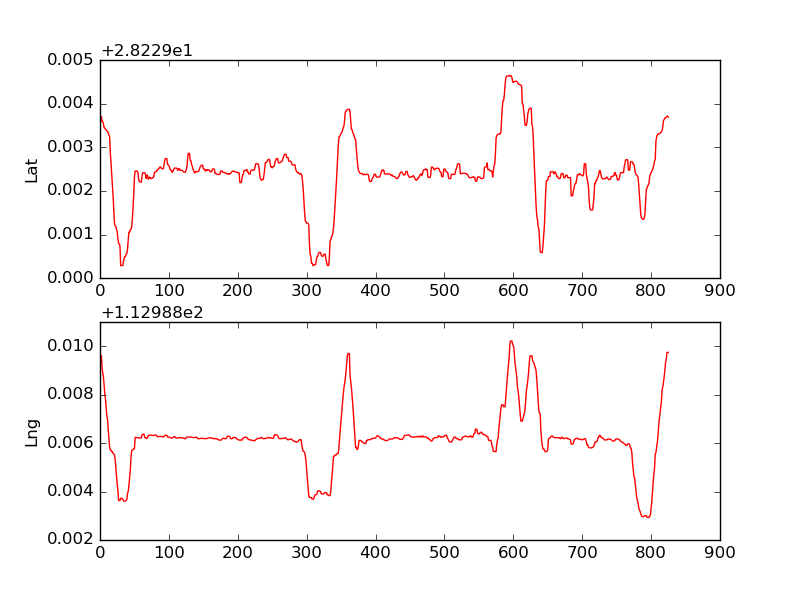
\includegraphics[height=4cm]{figure_4_mid_location2}}\hspace{4em}%
  \subfloat[分段卡尔曼滤波数据]{%
    \label{fig:3_2_2_2}
    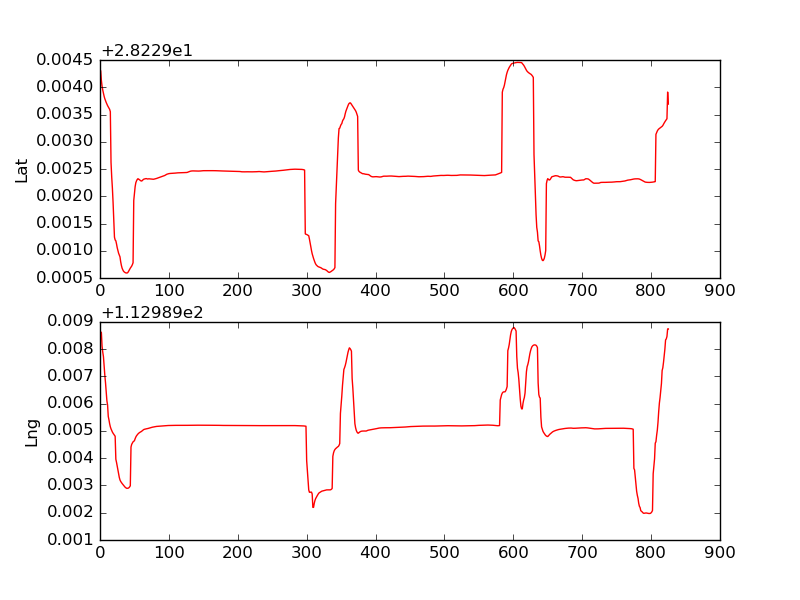
\includegraphics[height=4cm]{figure_4_mid_location2_kalman}}
  \caption{分段卡尔曼滤波轨迹结果2}
  \label{fig:3_5_2}
\end{figure}
\par 本小节主要针对前文中提及的三种常用的滤波算法进行了实验结果展示和效果分析,初步得出了使用卡尔曼滤波更加可行的判断结果。

\par 通过对停留点的识别,能够让我们更加深入的了解和认识用户的日常轨迹,同时从一个更加细粒度的层次来分析用户之间的轨迹相似度,停留点检测实验结果如图\ref{fig:SP_1}、\ref{fig:SP_2}所示,图中所得到的每一个停留点都具有丰富的现实意义,能够有效地表示用户访问的地点、位置。


---------------------------------------------------------
#停留点聚类
\par 第三层度量是基于用户手机的WiFi感知数据源,通过对WiFi感知数据的处理和结构化建模表示,本研究创新性的采用图结构来还原模拟出符合现实环境中某一时刻设备感知WiFi数据的周围的环境信息。因此在计算用户之间WiFi数据序列的相似度时,就将问题转换为计算每一个对应时刻内的WiFi感知上下文环境信息的相似度,进而来度量用户之间的社交关系强度。
\par 在第四层中用户关系度量是基于用户手机的蓝牙感知数据源,通过对蓝牙感知数据的处理和结构化建模表示,同样采用图结构来还原模拟出符合现实环境中某一时刻设备感知的蓝牙数据的周围的环境信息,在计算用户之间蓝牙数据序列的相似度时,就将问题转换为计算每一个对应时刻内的蓝牙感知上下文环境信息的相似度,进而来度量用户之间的社交关系度。
\par RSMHD模型从三种不同的数据源即用户日常轨迹、用户手机WiFi感知数据、用户手机蓝牙感知数据抽象出三种不同的层次度量模型,在基于用户轨迹度量层次中,又分解出三种度量维度,三种维度由低到高,由细粒度到粗粒度的度量使这一层次的计算结果更加有效和具有说服力,并最终根据这三层数据源的度量结果,借鉴集成学习的方法进行多层结果的融合。因此RSMHD以摒弃了单一的感知数据源采用多层数据源的用户关系计算并且最终对每层结果进行融合,能够更加有效全面的推理出现实生活中用户之间的社交关系强度。

